\documentclass[conference]{IEEEtran}
\IEEEoverridecommandlockouts
% The preceding line is only needed to identify funding in the first footnote. If that is unneeded, please comment it out.
%\usepackage{cite}
\usepackage{amsmath,amssymb,amsfonts}
\usepackage{algorithmic}
\usepackage{graphicx}
\usepackage{textcomp}
\usepackage{xcolor}
\usepackage{hyperref}
\usepackage[sorting=none]{biblatex}
\usepackage{algorithm}
\usepackage{dsfont}
% \usepackage{caption}
% \usepackage{subcaption}

\newcommand{\diff}[2]{\frac{d#1}{d#2}}
\newcommand{\pdiff}[2]{\frac{\partial#1}{\partial#2}}
\newcommand{\matt}[1]{\mathbf{#1}}
\newcommand{\vett}[1]{\boldsymbol{#1}}
\newcommand{\dvett}[1]{\dot{\boldsymbol{#1}}}
\newcommand{\ddvett}[1]{\ddot{\boldsymbol{#1}}}
\newcommand{\vers}[1]{\hat{\vett{#1}}}

\addbibresource{bibliography.bib}

\def\BibTeX{{\rm B\kern-.05em{\sc i\kern-.025em b}\kern-.08em
    T\kern-.1667em\lower.7ex\hbox{E}\kern-.125emX}}

\renewcommand{\epsilon}{\varepsilon}

\begin{document}

    \title{Neural network approximator for input allocation*\\
        {\footnotesize \textsuperscript{*}Final project for course \textit{Design Methods for Unmanned Vehicles}, prof.s D. Brunelli, D. Fontanelli, G. Moretti, L. Zaccarian.}
    }

    \author{
        \IEEEauthorblockN{Matteo Dalle Vedove}
        \IEEEauthorblockA{\textit{Department of Industrial Engineering} \\
            \textit{University of Trento, Italy}\\
            matteo.dallevedove@studenti.unitn.it
            }
        }


    \maketitle

    \begin{abstract}
        With this project I investigated the viability of using deep neural-networks to approximate a optimal allocation law.
        Tests have been carried out on the ROtor graSPing Omnidirectional (ROSPO) platform \cite{rospo} that provides a simple-enough, yet feature-full, testbed for propeller-driven vehicles.
        Experiments demonstrates the difficulty in accomplishing such task due to the high dimensionality of the function that needs to be approximated, showing that this approach is not satisfactory.
    \end{abstract}

    \section{Introduction}
When working with unmanned aerial vehicles, we usually deal with over-actuated systems. In fact even the simplest quadcopter can use different actuator configurations to achieve the same applied wrench to the center of mass.

More complex drones, such the one presented in \cite{hexarotor}, might use even more rotors that can be tilded by means of another servo motor, increasing the degree of overactuation in the system.

Whenever dealing with redundant actuation, key is to define an optimal way to distribute the load between the different components in order to accomplish the goal while minimizing a cost index that usually is the required actuation tower, in order to improve battery lifetime.

The goal of this project is to evaluate the performance that can be achieved when using neural networks for approximating the optimal control allocation of an over-actuated system.

To tackle this problem I used the ROtor graSPing Omnidirectional (ROSPO) platform \cite{rospo}, Fig. \ref{fig:rospomech}, a system developed at LAAS-CNRS to evaluate allocation scheme in propeller-driven vehicles. Such system has in fact the advantage of having a planar kinematics that simplifies the analytical burden of the system's dynamics, but presents all issues that must be addressed when working with drones.

\begin{figure}[b]
    \centering
    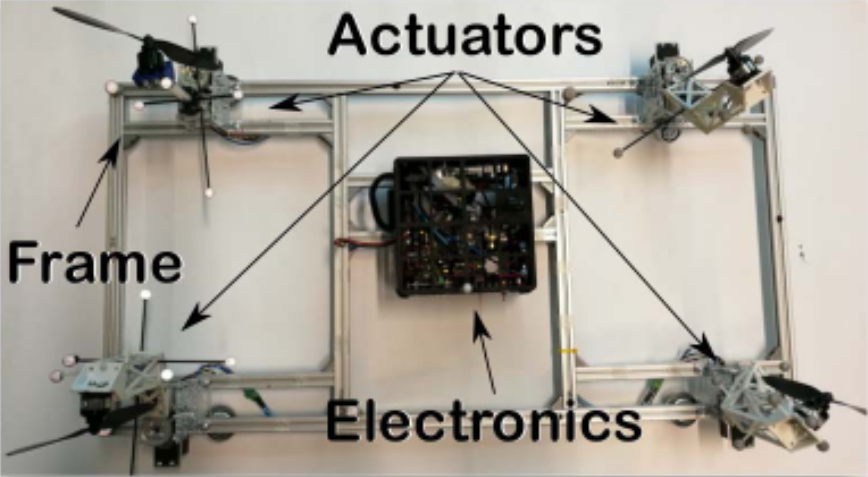
\includegraphics[width=5cm]{Images/rospo-paper}
    \caption{photo of the ROSPO prototype, courtesy of \cite{rospo}.}
    \label{fig:rospomech}
\end{figure}


The proposed idea is to use artificial neural networks trained offline on a dataset obtained by solving non-linear allocation problems; Khan et al. \cite{ANNallocator} reported promising results while solving allocation problem on an aerial vehicle, showing best regulation performance and lower evaluation time than common QP-based online solution.



This document will continue as follows: in Sec. \ref{sec:description} the ROSPO platform is described in more detail and its model is derived, Sec. \ref{sec:control} describes the control scheme that I used while Sec. \ref{sec:code} reports some implementation details. Later Sec. \ref{sec:results} reports some simulation results and finally conclusions are summarized in Sec. \ref{sec:conclusions}.

    \section{System description and modelling} \label{sec:description}

As described in \cite{rospo}, the ROSPO platform mainly consists in a rigid platform on top of which an arbitrary amount of actuator modules can be mounted. \\
Each of such module is a turret that is able to rotate on it's center with a stepper motor and on top of which a BLDC motor is used to drive propellers that will provide the thrust to move the system. \\
The moving frame is supported by means of omnidirectional passive spherical wheels.

\subsection{Motor modelling}
In contrast to what has been done in the reference paper, this simulation considers a more complex model of the BLDC motor that moves the propeller.

The proposed model is based on the equivalent single coil electrical circuit for the motor that's ruled by the following differential equation:
\begin{equation} \label{eq:singlecoil}
    L \diff{i} t = v - R\, i - e
\end{equation}
where $L, R$ are respectively the inductance and the resistance of the circuit, $i$ is the current flowing, $v$ is the voltage commanded to the circuit and $e$ is the back-electromotive voltage due to the rotation of the motor itself. Called such speed $\Omega$, it holds
\[ \Omega = k_{v} \, e \]

By balancing the electrical power dissipated by the BLDC motor with the resulting mechanical power, the output torque $T_{m}$ of the motor is
\[ T_{m} = \frac{i \, e}{J_{m}} \]
From the body mechanics, the differential equation ruling the angular speed of the rotor is
\begin{equation} \label{eq:rotordyn}
    J_{m} \diff{\Omega}{t} = T_{m} - T_{r}
\end{equation}
where $T_{r}$ is the (positive) resisting torque and $J_{m}$ is the motor's inertia (that comprises also the inertia of the propeller); given that the resisting torque is given just by aerodynamic actions, it can be approximated as $T_{r} = k_{r} \Omega^{2}$.

Combining (\ref{eq:singlecoil}) and (\ref{eq:rotordyn}) and removing the different algebraic constraints, leads to the following system of ODEs ruling the behavior of the BLDC motor:
\begin{equation} \label{eq:motordynamics}
\begin{cases}
    L \diff{i} t & = v - R \, i - \frac{\Omega}{k_{v}} \\
    J_{m} \diff{\Omega}t & = \frac{i}{k_{v}} - k_{r} \Omega^{2}
\end{cases}
\end{equation}
where $\Omega, i$ are the states of the system and $v$ is the input. Finally the force of the propeller $F_{p}$ is given by the state simply as
\begin{equation} \label{eq:motorforce}
    F_{p} = k_{l} \Omega^{2}
\end{equation}
where $k_{l}$ is the lift coefficient.

Numerically, all constants have been obtained, whenever possible, directly from datasheet of propellers and motors present in the laboratories; when data were not available, they have been derived considering simple mechanics. Table \ref{tab:motorcoeffs} report all such values.
\begin{table}[bt]
    \centering
    \caption{coefficients used in the motor's model.}
    \label{tab:motorcoeffs}
    \begin{tabular}{c c}
        constant & value \\ \hline \hline
        $k_{v}$ & $750 V / rpm$ \\
        $L$ & $27.2mH$ \\
        $R$ & $0.7 \Omega$ \\
        $k_{l}$ & $6.4\cdot 10^{-4}$ \\
        $k_{r}$ & $1.2\cdot 10^{-5}$ \\
        $J_{m}$ & $2.8\cdot 10^{-4} kg\cdot m^{2}$ \\
    \end{tabular}

\end{table}




\subsection{Friction force}
The reference model embeds also the effects of friction forces on the spherical wheels; the continuous function used is based on \cite{friction} and is of the form
\begin{equation} \label{eq:fricforce}
    \vett F_{f,\vett p}(\vett v) =
    \begin{cases}
        \mu(|\vett v|) \frac{\vett v}{|\vett v|} & \vett v \neq 0 \\
        0 & v = 0
    \end{cases}
\end{equation}
where $\vett v \in \mathbb R^{2}$ is the velocity of the point $\vett p$ in the plane and $\mu$ is the continuous function defined as
\[ \mu(s) = \gamma_{1}\big(\tanh(\gamma_{2}s) - \tanh(\gamma_{3} s)\big) + \gamma_{4} \tanh(\gamma_{5}s) + \gamma_{6} s \]

In the provided model $\gamma_{1}, \gamma_{2}, \gamma_{3}, \gamma_{6}$ are set to zero to neglect both Stribeck effect and viscous dissipation.
Since (\ref{eq:fricforce}) is continuous, it's time derivative later used in the control law can be computed as
\begin{equation} \label{eq:fricderivative}
    \dvett F_{r,\vett p}(\vett v) = \left(
        \left( \matt I  - \frac{\vett v \vett v^{\top}}{\vett v^{\top} \vett v} \right) \mu \big(|\vett v|\big)
        + \frac{\vett v \vett v^{\top}}{|\vett v|}\mu'\big(|\vett v|\big)
    \right) \frac{\dvett v}{|\vett v|}
\end{equation}
with
\begin{equation} \label{eq:mudt}
    \mu'(s) = \gamma_{4}\big(1 - \tanh^{2}(\gamma_{5}s) \big) \gamma_{5}
\end{equation}


\subsection{ROSPO modelling}
\begin{figure}[bt]
    \centering
    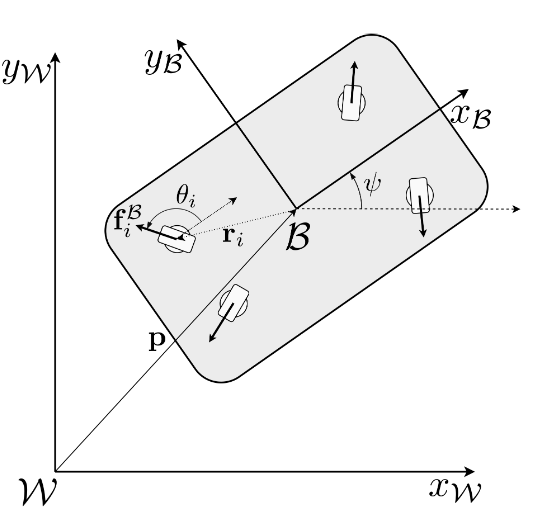
\includegraphics[width=5cm]{Images/rospo-scheme}
    \caption{schematic illustration of the ROSPO system; image courtesy of \cite{rospo}.}
    \label{fig:scheme}
\end{figure}
The ROSPO system is described as a single rigid body, i.e. the changes in mass and inertias due to the turrets rotations have been disregarded.
With this approximation in place the system's dynamic is described as
\begin{equation} \label{eq:dynamics}
\begin{cases}
    m \ddvett p_{com} & = \matt R(\psi)\sum_{i} F_{p,i} \vers u(\phi_{i}) + \sum_{i} \vett F_{r, \vett p_{i}} \\
    J \ddot \psi & = \sum_{i} \vett r_{i} \times F_{p,i} \vers u(\phi_{i}) + \sum_{i} \vett r_{\vett p_{i}} \times \vett F_{r, \vett p_{i}} \\
    \dot \phi_{i} & = \delta_{i}
\end{cases}
\end{equation}
where $\vers u(\phi_{i}) = \big(\cos(\phi_{i}), \sin(\phi_{i})\big)^{\top}$ represents the direction where the force $F_{p,i}$ of the $i$-th propeller is applied, with $\phi_{i}$ the relative orientation of the turret w.r.t the body's local frame that's described by an orientation $\psi$; $\vett r_{\circ}$ are instead the vectors describing the distance of the point where the force is applied w.r.t. the center of mass of the ROSPO; finally $m,J$ are the mass and the inertia of the system. \\
The rotation matrix \[ \matt R(\psi) = \begin{bmatrix} \cos \psi & -\sin\psi \\ \sin\psi & \cos\psi \end{bmatrix} \]
is used to convert the force computed in the local frame of the body into the inertial ground reference frame. \\
The dynamics of the turret's attitude $\phi_{i}$ is linear w.r.t. the corresponding input $\delta_{i}$ since such element is moved by a stepper motor.

After reducing the system to a first order ODE the states $\vett x$ and input $\vett u$ are:
\begin{equation} \label{eq:states}
\vett x =
\begin{pmatrix}
    x_{com} \\ y_{com} \\ \psi \\ v_{x,com} \\ v_{y, com} \\ \omega \\
    \Omega_{1} \\ i_{1} \\ \phi_{1} \\ \vdots \\ i_{N_{t}} \\ \phi_{N_{t}}
\end{pmatrix} \in \mathbb R^{6 + 3N_{t}}
\qquad \vett u =
\begin{pmatrix}
    v_{1} \\ \delta_{1} \\ \vdots \\ v_{N_{t}} \\ \delta_{N_{t}}
\end{pmatrix} \in \mathbb R^{2N_{t}}
\end{equation}
where $N_{t}$ is the number of turrets installed on the ROSPO platform that for the following simulation is chosen to $4$.


    \section{Control} \label{sec:control}
The control scheme developed is similar to the one proposed in \cite{rospo} that exploits an hierarchical control architecture with an high level controller responsible to convert the system's state and the respective desired motion into a virtual wrench that's desired on the center of mass (com), and an allocator that dispatches the loads into the different turrets to achieve the goal.

\subsection{High level controller}
The high level controller used in this project is the one derived in \cite{rospo} and is developed so that the controller sees an equivalent first-order linear dynamics.

The commanded virtual input $\vett u_{v,c}$, i.e. the desired wrench on the com of the ROSPO, is computed by the law
\begin{equation} \label{eq:virtualinput}
    \vett u_{v,c} = \matt B^{-1} \big( \dvett u_{v}^{\star} - \matt A \vett u_{v}^{\star}\big) - \matt K \tilde{\vett u}_{v}
\end{equation}
with $\matt A = -\gamma_{P} \matt I_{3}$, $\matt B = \gamma_{P} \matt I_{3}$ and $\matt K\in \mathbb R^{3\times 3}$ a gain matrix such that $\matt A - \matt{BK}$ is Hurwitz. In (\ref{eq:virtualinput}) the feedforward signal and it's time derivative are
\begin{align*}
\vett u_{v}^{\star} & = \begin{pmatrix}
    m \matt R^{\top}(\psi) \left( -k_{p} \tilde{\vett p} - k_{d}\dot{\tilde{\vett p}} + \ddvett p_{ref} - \frac{\vett F_{f}(\vett x)}{m} \right) \\
    J \left( -k_{p, \psi} \tilde{\psi} - k_{d,\psi}\dot{\tilde{\psi}} + \ddot \psi_{ref} - \frac{T_{f,\psi}(\vett x)}{J} \right)
\end{pmatrix} \\
\dvett u_{v}^{\star} & = \begin{pmatrix}
    m \matt R^{\top}(\psi) \big( \matt S(\psi) \vett v + \vett v_{d} \big) \\
    J \left( -k_{p, \psi} \dot{\tilde{\psi}} - k_{d,\psi}\ddot{\tilde{\psi}} + \dddot \psi_{ref} - \frac{\dot T_{f,\psi}(\vett x)}{J} \right)
\end{pmatrix}
\end{align*}
with $k_{\circ}$ all positive gains, $\vett F_{f}, T_{f,\psi}$ respectively the force and the torque due to the friction (as function of the current state of the ROSPO), and $\tilde{\vett p} = \vett p - \vett p_{ref}$ the position error w.r.t. the reference trajectory described by $\vett p_{ref}$. Finally
\begin{align*}
\matt S(\psi) & = \begin{bmatrix}
    0 & \dot \psi \\ -\dot \psi & 0
\end{bmatrix} \\
    \vett v & = -k_{p} \tilde{\vett p} - k_{d} \dot{\tilde{\vett p}} + \ddvett p_{ref} - \frac{\vett F_{f}}{m} \\
    \vett v_{d} & = -k_{p} \dot{\tilde{\vett p}} - k_{d} \ddot{\tilde{\vett p}} + \dddot{\vett p}_{ref} - \frac{\dvett F_{f}}{m}
\end{align*}


\subsection{Allocator}
Most of the effort for the project has been put into the development of the allocator whose goal is to convert the commanded virtual input $\vett u_{v,c}$ into a set of proper inputs $\vett u$ for the system.

In the reference paper, such task is accomplished exploiting the system's model by using an input that guarantees an optimal regulation as well as asymptotic optimality condition; due to the nature of such problem, no saturation or boundaries on the inputs can be ensured, but they are regarded as soft constraints by properly choosing the cost function.

The idea that I propose is instead to use deep neural networks to approximate the optimal input allocation; based on the system's model, a dataset of optimal allocations can be computed offline and used to train the neural network that later can be used only in prediction while running on the effective system. \\
With this approach computationally expensive algorithms can be used offline to accomplish the allocation while at runtime a deterministic computation of the input is guaranteed by the evaluation of the neural network.

The developed allocation method relies on 2 stages that exploits different neural networks: the first one performs the proper allocation by computing the force (with its attitude) that each turret should have at the next controller update (based on the current state and the commanded virtual input) and a lower-level controller that converts the desired force into a voltage to be applied at the BLDC motors. For sake of simplicity the latter one is described first. \vspace{3mm}

\subsubsection{BLDC voltage identification}
To compute the voltage $v$ that allows to reach a desired force $F_{des}$, model (\ref{eq:motordynamics}) is used.

Since $v$ doesn't appear explicitly in (\ref{eq:motorforce}), the force $F$ generated by the model can't be instaneously changed by choosing the voltage; for this reason a discrete approach has been used: given the initial state $\vett x_{0} \in \mathbb R^{2}$ of the motor, the ODE is numerically integrated using Runge Kutta methods to determine the force $F^{+}$ at the next cycle of the controller. With this idea the optimal control $v^{\star}$ is given by
\begin{equation} \label{eq:optimalvoltage}
    v^{\star}(\vett x_{0}) = \arg \min_{v} \big\|F^{+}(v, \vett x_{0}) - F_{des}\big\|^{2}
\end{equation}

To improve the convergence of numerical methods, the explicit definition of the jacobian of the cost w.r.t. the decision variable $v$ has been provided; rewriting in fact the cost as
\[ c = \big(F^{+} - F_{des}\big)^{\top} \big(F^{+} - F_{des}\big)\]
it turns out that
\[ \diff c v = 2 \big(F^{+} - F_{des}\big) \pdiff{F}{\vett x} \diff{\vett x}v \]
where $\diff{\vett x}v$ can be obtain by computing the sensitivities with the Runge Kutta methods.

The dataset for computing the input voltage to the motor has been generated from solving (\ref{eq:optimalvoltage}) by uniformly sampling $\vett x_{0} \in \mathcal X \subset \mathbb R^{2}$ on a set of bounded values for the state and constraining $v\in [0,v_{max}]$. \\
To increase the quality of the dataset, data have been generated also considering $\vett x_{0}$ as a small deviation from a steady-state configuration.
\vspace{3mm}

\subsubsection{Allocation}
The dataset for the allocator neural-network has been developed similarly to the previous case, i.e. by solving constrained least-square problems on state uniformly sampled from a defined subspace.

For this problem let's consider the state $\vett x \in \mathbb R^{2N_{t}}$ the one defined as
\[ \vett x = \Big( F_{1}, \phi_{1}, \dots, F_{N_{t}}, \phi_{N_{t}}\Big)^{\top} \]
while $\vett u \in \mathbb R^{2N_{t}}$ is simply the ratio of change in time of the respective variables, i.e.
\[ \vett u = \Big( \delta F_{1}, \delta\phi_{1}, \dots, \delta F_{N_{t}}, \delta\phi_{N_{t}}\Big)^{\top} \]

Defined with $\vett F_{com}(\vett x): \ \mathbb R^{2N_{t}} \rightarrow \mathbb R^{3}$\footnote{In this case we implicitly assume that the force is a 3-dimensional vector with the 3rd component being the applied torque.} the function that given the current state provides the wrench applied to the com, then the minimization problem to solve is of the form
\begin{equation} \label{eq:allocproblem}
\begin{aligned}
    \vett u^{\star} (\vett x_{0}) = \arg \min_{\vett u} & \big\|\vett F_{com}(\vett x_{0} + T_{s}\vett u) - \vett F_{des} \big\|^{2}_{\matt W_{1}} \\ & + k \| \vett u \|^{2}_{\matt W_{2}}
\end{aligned}
\end{equation}
The reported cost function have 2 main contributions: the first one is used to regulate the input toward the desired wrench, while the second one minimizes the actuation effort. In both cases the least-square costs are weighted by matrices $\matt W_{\circ}$ in order to improve the control selection.

Also in this case a subset for both $\vett F_{des}$ and $\vett x_{0}$ is defined; the dataset is built by randomly sampling from those spaces and solving problem (\ref{eq:allocproblem}) considering boundaries on $\vett u$.

    \section{Implementation details} \label{sec:code}
Implementation-wise, the project has been developed using different tools.

Main symbolic computation has been carried out using the software \textit{Maple} \cite{maple}. With the help of integrated C code generation of the software, an additional library has been developed to convert all symbolic function into \textit{C++} function for faster evaluation, using the \textit{Eigen} \cite{eigen} linear algebra library as backend; furthermore the utility create wrapper code for all functions for the python language using \textit{pybind11} \cite{pybind11}, with a script that automatically creates necessary dynamic libraries.

Numerical evaluations have been carried out in python; optimization problems have been solved using utilities from the \textit{scipy} \cite{scipy} library, while \textit{tensorflow} \cite{tensorflow} has been used to train deep neural-network models.

Deep-learning models tested have been fully-connected neural networks with different amount of hidden layers and corresponding sizes; the chosen activation function for each perceptron is the rectified linear unit (\textit{ReLU}), since it's less prone to the vanishing gradient problem \cite{vanishing}.

All the source code is freely available at \url{https://github.com/matteodv99tn/UAV-project}.

    \section{Results} \label{sec:results}
With the code developed, several tests have been performed to assess the viability of the proposed solution. Even if the underlying idea of fitting functions using neural networks seems interesting, evidence shows non-promising results.

The main issue can be related to the dataset generation and model training. Considering a case with 4 turrets, the goal is to fit a function $\vett f:\ \mathcal X \subset \mathbb R^{11} \rightarrow \mathbb R^{3}$; to have a good and reliable approximation, the whole space $\mathcal X$ should be \textit{sufficiently visited} from a numerical standpoint.

Working from my laptop, even tough minimization problems can be solved as fast as $1ms$, generating $1\,000\,000$ data points requires almost 30 minutes; furthermore with such generated data, each deep-learning model requires about 1 hour to train over 100 epochs. \\
With such amount of data, still the process of training the neural network fails to achieve satisfactory results, probably due to the lack of data that enables a proper function fitting.

\vspace{3mm}
The potentiality of the tool is well expressed when controlling the voltage to be applied to the BLDC motor; such problem requires the fitting of a function $f:\ \mathcal X \subset \mathbb R^{3} \rightarrow \mathbb R$ with a domain of smaller size for which the computation of a sufficiently large data-set is viable.

As exposed in Fig. \ref{fig:motorNN}, models with different configurations of hidden layers are able to reach and correctly track the reference trajectory asked the system.
\begin{figure}[bt]
    \centering
    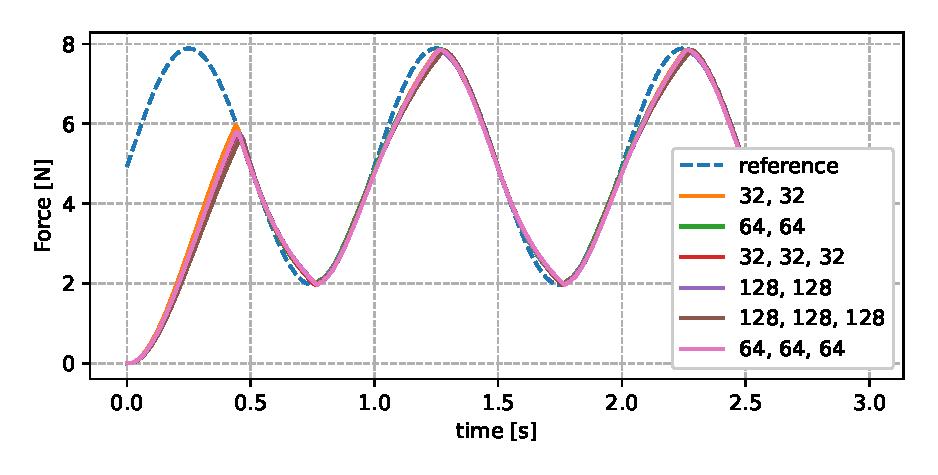
\includegraphics[width=\linewidth]{Images/motorNN.eps}
    \caption{response of different controllers to a sinusoidal input. For each model the number of perceptron in each hidden layer is reported, e.g "32, 32" means \textit{2 hidden layers with 32 perceptrons each}.}
    \label{fig:motorNN}
\end{figure}

\vspace{3mm}

Using one of the above models and solving the allocation problem (\ref{eq:allocproblem}) at each control step shows the desirable behavior in a trajectory-tracking scenario. Considering the 8-shaped trajectory described by
\[ \vett p =
\begin{pmatrix}
    \rho_{x} \cos(c_{1} t) \\ \rho_{y} \sin(c_{2}t) \\ 0
\end{pmatrix}
\]
then Fig. \ref{fig:path} shows the path followed by the ROSPO considering simulation parameters in Table \ref{tab:simdata} and having chosen the feedback matrix $\matt K$ for which the eigenvalues of the close-loop matrix $\matt A - \matt{KB}$ are $(-3,-3,-3)$. Figure \ref{fig:error} reports a more detailed look at the time behavior of the different $x, y$ and $\psi$ component of the state. Finally, Fig. \ref{fig:force} shows how the allocator responds to the commanded virtual input.

\begin{table}[bt]
    \centering
    \caption{coefficients used in the ROSPO simulation.}
    \label{tab:simdata}
    \begin{tabular}{c c}
        parameter & value \\ \hline \hline
        $\rho_{x}$ & $1m$ \\
        $\rho_{y}$ & $0.6m$ \\
        $c_{1}$ & $0.4$ \\
        $c_{2}$ & $0.8$ \\
        $\gamma_{P}$ & $2.5$ \\
        $k_{p}$ & $1.2$ \\
        $k_{d}$ & $1.4$ \\
        $k_{p, \psi}$ & $3.2$ \\
        $k_{d, \psi}$ & $6.35$ \\
        $\gamma_{4}$ & $0.44$ \\
        $\gamma_{5}$ & $1$ \\
        $m$ & $6kg$ \\
        $J$ & $6.1kg\cdot m^{2}$
    \end{tabular}
\end{table}


\begin{figure}[bt]
    \centering
    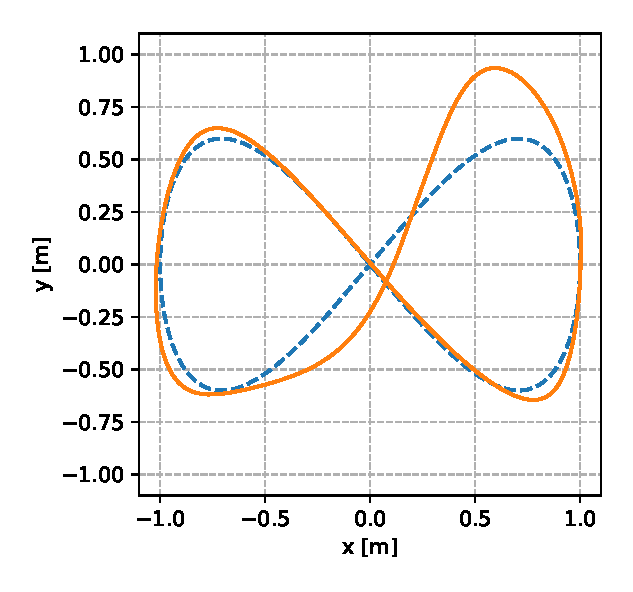
\includegraphics[width=5cm]{Images/path.eps}
    \caption{path followed by the ROSPO while prompted to follow the 8-shaped trajectory.}
    \label{fig:path}
\end{figure}
\begin{figure}[bt]
    \centering
    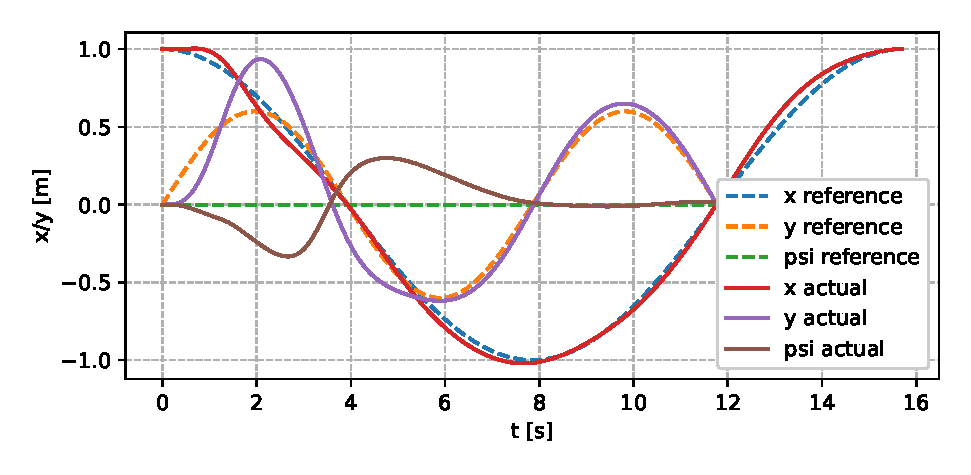
\includegraphics[width=\linewidth]{Images/delta.eps}
    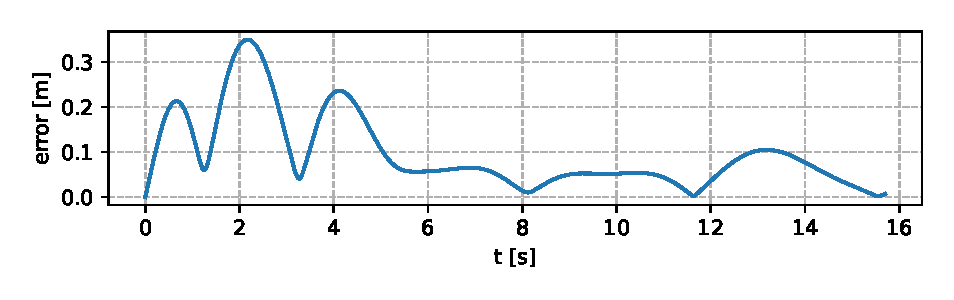
\includegraphics[width=\linewidth]{Images/error.eps}
    \caption{desired and actual position and orientation of the ROSPO during the simulation.}
    \label{fig:error}
\end{figure}
\begin{figure}[bt]
    \centering
    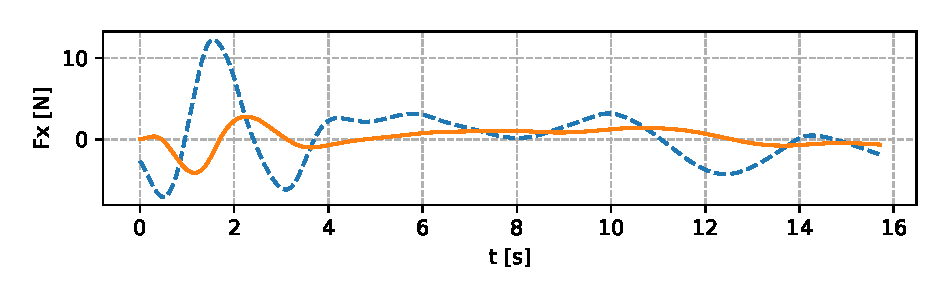
\includegraphics[width=\linewidth]{Images/force-1.eps}
    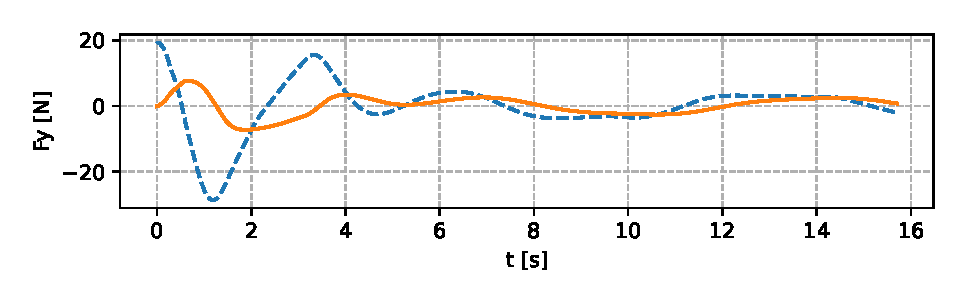
\includegraphics[width=\linewidth]{Images/force-2.eps}
    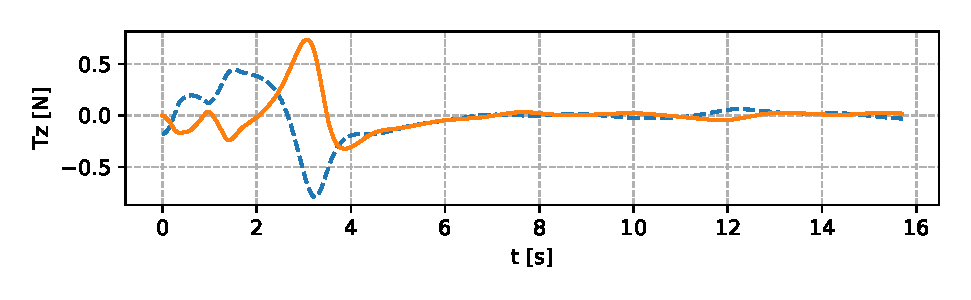
\includegraphics[width=\linewidth]{Images/force-3.eps}
    \caption{commanded virtual input and actual force exherted by the system as function of time in the cardinal directions and resulting torque.}
    \label{fig:force}
\end{figure}

At the beginning, due to a standstill initial condition, the controller isn't capable of following the requested trajectory, and goes into severe errors while following the path; toward the end instead the system converges to the desired trajectory as expected.

    \section{Conclusions} \label{sec:conclusions}
As discussed in the previous section, it can be concluded that using deep neural networks to approximate the optimal allocation law is not feasible, at least with the developed procedure. \\
The problem of dimensionality will be even higher in case of aerial UAVs, with 3-dimensional space of motion and a higher amount of actuators.

Leaning toward data-driven control methods, interesting could be to develop a reinforcement learning allocator: such technique is based on collected experience by the system itself: this might reduce the exploration of the state space mainly to relevant subspaces, and the learning process is performed online with incremental steps.

As final notes, two points are still open for evaluation:
\begin{itemize}
    \item comparing the allocation results with the one provided in the reference paper; in this case the model of the BLDC motor has been developed more in detail, and a review of the presented theory in \cite{rospo} is required; alternatively one could also use a lower-level controller to compute the voltage given the speed reference as in that paper;
    \item developing a more complex model that takes into account for uncertainties: both high level controller and allocator use at each timestep the values computed by the simulator, so the system is fully observable and behaves deterministically. Interesting should be an approach where the dataset is built from the deterministic model, but testing is carried out by faking measurement comparable with a real world scenario and using state estimators to reconstruct the actual state of the system.
\end{itemize}



    \printbibliography



\end{document}

